\documentclass[10pt,a4paper]{report}
\usepackage[latin1]{inputenc}
\usepackage{amsmath}
\usepackage{amsfonts}
\usepackage{amssymb}
\usepackage{graphicx}
\usepackage{pdfpages}
\usepackage{listings}
\lstset{tabsize=4}

\title{CS325 HW2}
\author{Brock Smedley}
\begin{document}
	\maketitle
	
	\section*{1}
	
	\subsection*{a)}
	T($n$) is $\Theta(2^n)$.
	\\
	
	$T(n) 	= 2T(n-2) + 1$
	
	$		= 2(2T(n-4) + 1) + 1$
	
	$		= 2T(2T(2T(n-6) + 1) + 1) + 1$
	
	$		= 2T(2T(2T(...2T(0|1)...+1)+1)+1)+1$

	Function recurses n times, each time adding 1 and multiplying each successive result by 2.

	$T(n)	= O(2^n + n) \implies \Theta(2^n)$
	
	\includegraphics*[scale=0.5]{1a}
	
	Green: $2^n + n$
	
	Blue: $2^n$
	
	Red: $0.9*2^n$
	
	\subsection*{b)}
	T($n$) is $\Theta(n^4)$. 
	\\
	
	$T(n) 	= T(n-1) + n^3$
	
	$		= T(n-2) + (n-1)^3$
	
	$		= T(n-3) + (n-2)^3$
	
	$		= 1 + ... + (n-2)^3 + (n-1)^3 + n^3$
	
	$		= \sum_{i=1}^{n} n^3 = \Theta(n^4)$
	
	\newpage
	\subsection*{c)}
	Master method:
	
	$T(n) = 2T(n/6) + 2n^2$
	
	$a = 2$
	
	$b = 6$
	
	$f(n) = 2n^2$
	\\
	
	$f(n) = \Omega(n^{log_b(a+\epsilon)})$ for $\epsilon = 1$.
	
	\includegraphics*[scale=0.5]{1c}
	
	Green: $n^{log_b(a+\epsilon)}$
	
	Blue: $n^2$
	\\
	
	$a*f(n/b) < c*f(n)$
	
	$\implies 2*f(n/6) < c*f(n)$; let c = 0.25.
	
	$\implies 2*2(n/6)^2 < 0.25*2n^2 \implies 4(n/6)^2 < 0.5n^2$
	
	\includegraphics*[scale=0.5]{1c2}
	
	Green: $0.5n^2$
	
	Blue: $4(n/6)^2$
	\\
	
	Solution: $T(n) = \Theta(f(n)) = \Theta(2n^2) = \Theta(n^2)$
	
	\newpage
	\section*{2}
	\subsection*{a)}
	The quaternary search function takes arguments for the search parameter, the array, and the left and right indices.
	
	The algorithm starts by checking for a base case; that the size of the array bounds defined by the left and right index arguments is $\le$ 4. If the base case is met, then the function simply scans the subarray until it finds x, or returns -1 if it doesn't find it. This portion is $O(4)$.
	
	If the base case is not met, then the function splits the array into four roughly equal parts; it defines the quaternary boundaries using the left and right indices to calculate middle-left, middle, and middle-right (left and right implicitly included in the boundaries). I refer loosely to the bounds, which these indices define, as "subarrays." Each recursive iteration yields four new subarrays, of which the function's array parameter was initially comprised.
	
	After defining "end indices" of our subarrays, the algorithm scans the right index of each quaternary boundary (middle-left, middle, middle-right, right) to find a number $\ge$ x. If such a number is found, we recursively call the function with that subarray as the new left and right boundaries.
	
	This method allows us to cut the size of our search domain by a factor of 4 for each iteration, with the caveat that we have to do up to 4 comparisons for each recursive level to find the bounds of that level.
	\\
	
	\newpage
	Pseudocode:
\begin{lstlisting}
// returns index of element in arr equal to x
function qSearch(arr, left, right, x){
	// base case: (sub)array down to 4 or less elements
	if (right-left < 4){
		# check elements of arr[left:right] for x
		for i in range(left, right){
			if (arr[i] == x)
				return i
		}
	
		return -1 # didn't find element
	}
	
	// recursive case: split array into 4 pieces
	// assume integer division (floor) to calculate indices
	mid = l + (right-left)/2
	ml = (mid - left)/2
	mr = (right - mid)/2 + mid
	
	// store indices for later iteration
	indices = [left, ml, mid, mr, right]
	
	// find subarray containing x; scan boundary ahead for n > x
	for i in range(len(indices)-1){
		if (arr[indices[i+1]] >= x) // x should be in this subarray
			return qSearch(arr, indices[i], indices[i+1], x)
	}
	
	return -1 // element not in any subarray
}
\end{lstlisting}
	
	\newpage
	\subsection*{b}
	$T(n) = n$ if $n \le 4$
	
	\noindent
	$T(n) = T(n/4) + 4$ if $n > 4$
	
	\subsection*{c}
	Assuming $n > 4$, $T(n) = T(n/4) + 4$
	
	$T(n/4) = T(n/16) + 4$
	
	$T(n/16) = T(n/64) + 4$
	
	\dots
	
	$T(n) = O(4log_4(n)) = \Theta(4log_4(n))$
	\\
	
	While the running time analysis implies that this algorithm runs in $O(log_4(n))$ time, which is faster than $O(log_2(n))$ it's actually slower than a traditional binary search. This is because we have to include the 4x multiplier to include the four potential comparisons to find the next subarray. Traditional binary search algorithms only have to make up to two comparisons ($\le$ or $>$). 
	
	If we were to change the algorithm to only scan the middle and right boundaries to find the next subarray, we could try to match the speed of a binary sort, but that's only because we're actually just implementing a binary search with more identifiers. At any rate, in this hypothetical example, we would still have to scan two boundaries, so our efforts to optimize would be futile.
	
	\newpage
	\section*{3}
	\subsection*{a}
	This algorithm finds the minimum and maximum values in an unsorted array by splitting the list in half and recursively evaluating the min/max values of the subarrays. The first two recursive cases split the array in half and recurse until the base case is reached. This happens twice, one for each side.
	
	When the function detects that the array is of size $2 \le n \le 3$ (base case), it manually evaluates the minimum and maximum and sorts the two-to-three-element subarray, which the function then returns. When the second recursive call returns, the recursive "parent," so to speak, determines the two min/max numbers from the two pairs that were just returned. Lastly, it returns a recursive call to itself with the two-element pair it just created. This will trigger the base case and merge the data to eventually land at the global min/max pair.
	\\
	
	\noindent
	Pseudocode:
	
	\begin{lstlisting}
function minmax(arr){
	// base case: array is < 4, we can manually find min/max
	if (len(arr) < 4 && len(arr) > 1){
		min = arr[0]
		max = arr[1]
		// verify min/max, assign to appropriate index
		if (min > max){
			max = min
			min = arr[1]
		}
		// handle potential 3rd element
		if (arr[2]){
			if (arr[2] > max)
				max = arr[2]
			elif (arr[2] < min)
				min = arr[2]
		}
		
		return [min,max]
	}
	elif (len(arr) == 1)
		return [arr[0],arr[0]]
	else{
		// recursive case: array size > 2
		// split array and find min/max recursively
		mid = len(arr)/2
		left = minmax(arr[0:mid]) # colon means "to, inclusive"
		right = minmax(arr[mid+1:-1]) # -1 is last element
		min = math.min(left[0], right[0])
		max = math.min(left[1], right[1])
		return minmax([min,max])
	}
}
	\end{lstlisting}

	\newpage
	\subsection*{b}
	$T(n) = 2T(n/2) + O(n)$ if $n > 1$
	\\
	$T(n) = 1$ if $n = 1$
	
	\subsection*{c}
	$T(n) = \Theta(n lg n)$
	
	The running time of this algorithm is $n lg n$ because the algorithm has to recursively traverse the tree $lg n$ times, then at the base case level, does a sum total of n operations. An iterative algorithm would run in $\Theta(n)$ time, which is faster than $\Theta(n lg n)$. 
	
	This type of algorithm would make much more sense to do iteratively since, no matter what, we have to read every element in the array. Obviously, the iterative algorithm would simply read every element in the array and compare it to some saved values for min/max, updating the respective values as it progressed through the array, making a total of n comparisons.
	
	\newpage
	\section*{4}
	\subsection*{a}
	The StoogeSort function is a recursive algorithm whose base case is for the array A to be of length 2. When the base case is satisfied, the algorithm swaps the elements if they are out of order, or leaves them alone otherwise.
	
	The algorithm reaches the base case by whittling down the size of the array using $ceiling(2n/3)$ to calculate an index (somewhere in the middle-ish area of A) which splits the array recursively. Once the base case is reached and the two "base elements" are in order, the first call of the function returns. Then, the algorithm makes another recursive call to sort the rest of the given subarray recursively, excluding the leftmost element which has just been sorted. Once that call chain returns, a last call is made to re-sort the first part array which may have been modified during the last call chain.
	
	\subsection*{b}
	No, StoogeSort would not correctly sort if we replaced $k=ceil(2n/3)$ with $k=floor(2n/3)$. When $n = 4$, the algorithm ends up returning a one-element array in the recursion stack. The reason this doesn't work is because the algorithm doesn't have a base case for $n = 1$, so the algorithm would continue making recursive calls infinitely and you would get a "maximum recursion depth exceeded" error, or something like that.
	
	\subsection*{c}
	$T(n) = 2T(2n/3 - 1) + T(n - 2n/3 + 1)$
	
	\subsection*{d}
	$T(n) = 2T(2n/3 - 1) + T(n - 2n/3 + 1)$
	
	$	\implies O(2^n + n)$
	
	$	= \Theta(2^n)$
	
	\newpage
	\section*{5}
	\subsection*{b}
	\begin{lstlisting}
# stoogesort_test.py
# Brock Smedley 2018

import math
import sys
from random import randint
import timeit

# modifies array in place
def stooge(arr, l, r):
	if (l >= r):
		return
	
	if (arr[l] > arr[r]):
		temp = arr[r]
		arr[r] = arr[l]
		arr[l] = temp
	
	if ((r - l + 1) > 2):
		m = int(math.ceil((r - l + 1) / 3.0))
		stooge(arr, l, r-m)
		stooge(arr, l+m, r)
		stooge(arr, l, r-m)


# returns array[n] of random data
def readData(n):
	data = []
	for i in range(n):
		data.append(randint(1,1000))
	
	#print "unsorted data: \t" + str(data)
	return data

\end{lstlisting}
\begin{lstlisting}
# accepts list of [n, run-time] pairs, writes each into a csv
def writeData(data):
	f = open("data.out", "w")
	f.write("n \t time \n")
	i = 0
	for d in data:
		dw = str(d[1])
		n = str(d[0])
		f.write("%s \t %s"%(str(n) ,str(dw)))
		if (i < len(data)-1):
			f.write("\n")
		i += 1


# test the stoogesort
def test():
	m = 1600
	r = 20
	w = m / r
	times = []
	for i in range(r):
		n = (i+1)*w
		#print "n: " + str(n)
		data = readData(n)
		t = timeit.default_timer()
		stooge(data, 0, n-1)
		d = timeit.default_timer() - t
		times.append([n, d])
		#print ("running time: %s seconds" % str(d))
	writeData(times)
	#print "sorted array: \t" + str(data)

test()
	\end{lstlisting}
	
	\newpage
	\subsection*{c}
	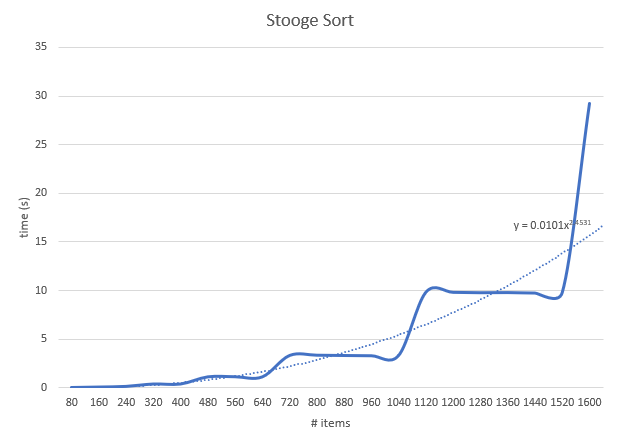
\includegraphics[scale=0.6]{stooge}
	
	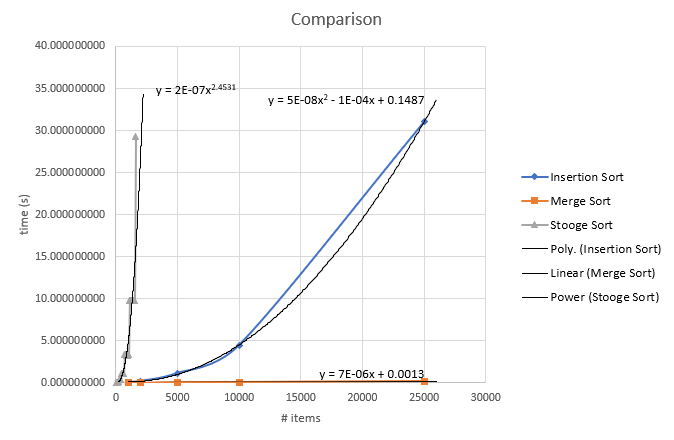
\includegraphics[scale=0.8]{comparison}
	
	\newpage
	\subsection*{d}
	The StoogeSort data set appears to resemble an polynomial (power function) curve. The time resolution on my computer was less-than-accurate when I ran these tests, but the data is sufficient to illustrate the trend of the data. If we Google "Stooge Sort complexity," we'll find that Stooge sort is indeed a polynomial function; $O(n^{2.7095...})$ to be exact. You'll notice that the equations for the trend lines differ per chart; that is because the charts have different domain sizes -- there is no way I could sort 30,000 numbers with StoogeSort in a reasonable amount of time.
	
	The theoretical time (some $n^c$) appears to be a little higher than the actual experimental time, but that is probably due to poor data resolution. Looking at the data on the Comparison chart best illustrates the similarities in running-times.
	
\end{document}